\section{Methodology and workplan}
% [max 1.5 page]

%Provide: 
%	\item[-] Overview of the proposed approach you plan to follow (including methods and techniques)
%	\item[-] List of tasks organized in tables (see below). (For each task, brief summary of the progress of the research accomplishments (the details about the results achieved will be provided in Sect. 4).
%	
%	Additionally, a Gantt chart is required (see below for an example).

\begin{figure}[H]
	\centering
	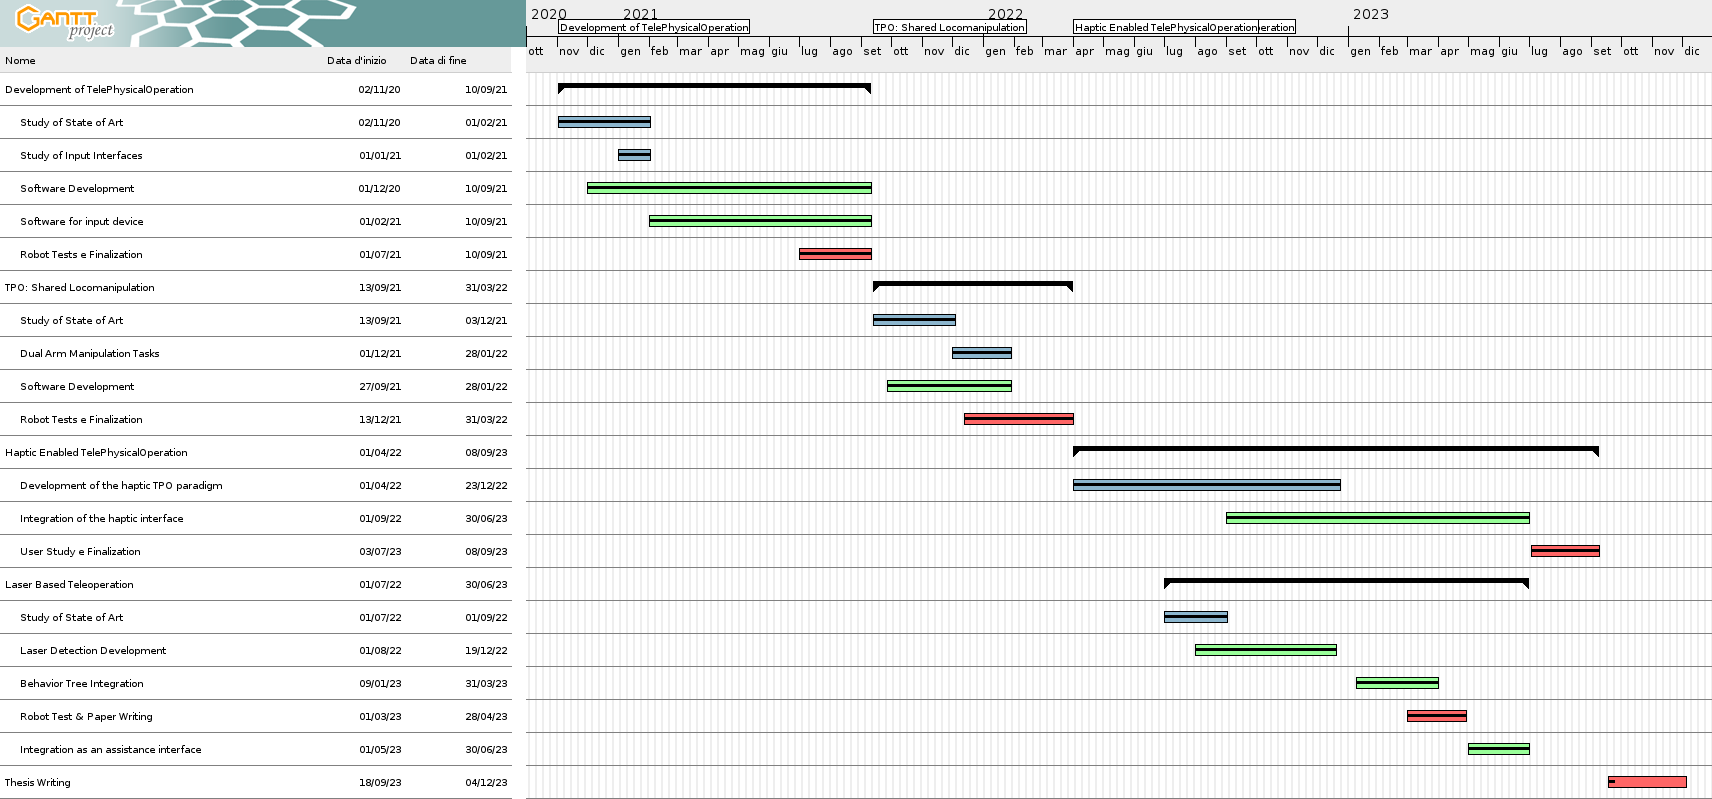
\includegraphics[width=1\linewidth]{img/PHD_thirdYear}
	\caption{Gantt chart displaying the relevant tasks}
	\label{fig:phdthirdyear}
\end{figure}



To advance the state of the art in telerobotics, this research addressed the key challenges of enabling effortless control of complex robots by developing intuitive interfaces which include robot autonomy features.
In the first period, the TelePhysicalOperation interface has been developed. Later, the interface has been enhanced with some robot autonomy features to \enquote{share the control} between the operator and the robot itself: for example, while the operator commands only the velocity of the end-effector, the robot generates arm commands and mobile base commands according to the arm manipulability level, letting the end-effector to reach the goal even if it is out of the reaching of the arm.
The interface has been further enriched by incorporating a haptic feedback channel, allowing users to perceive information beyond the visual domain. Naive users who evaluated the haptic-enabled TelePhysicalOperation positively endorsed the inclusion of haptic cues.

Concurrently, an alternative teleoperation interface has been developed, utilizing visual servoing guidance with a laser device. The resulting user interface is very easy-to-use and intuitive, permitting to the user to indicate location of interest with an inexpensive device. Nevertheless, this has required more robot autonomy which has been addressed with an architecture based on Behaviour Trees~\cite{Iovino2022}.
Other than with complex robots, the interface has been evaluated with a simpler fixed manipulator, showing the potentiality of this interface as an assistive device for impaired arm users.
	
\begin{table}[H]
	\begin{center}
		\renewcommand{\arraystretch}{1.3} % Adjust the vertical spacing
		\setlength{\tabcolsep}{8pt} % Adjust the horizontal spacing
		\begin{tabular}{|P{15cm}|}
			\hline
			\textbf{Task name} Development of TelePhysicalOperation (TPO) \\ \hline
			\textbf{Scheduling}: Months 1-11 \\ \hline
			\textbf{Performed actions}: Studied the state of art regarding teleoperation, human-robot interaction, and leader-follower hardware interfaces. 
			Developed Software Architecture for both control part and input interface 
			Evaluation experiments on real robot\\
			\hline
			\textbf{Achieved results}: A Control Interface to teleoperate complex robot has been developed. Test on real platform (CENTAURO) has been validated, resulting in a publication. Presentation at the ICRA22 conference \\
			\hline
			\textbf{Status}: Completed\\
			\hline
			\textbf{Publications relative to the task}: [J.1]\\
			\hline
			\textbf{Revised planning}\\
			\hline
		\end{tabular}
	\end{center}
\end{table}

\begin{table}[H]
	\begin{center}
		\renewcommand{\arraystretch}{1.3} % Adjust the vertical spacing
		\setlength{\tabcolsep}{8pt} % Adjust the horizontal spacing
		\begin{tabular}{|P{15cm}|}
			\hline
			\textbf{Task name} TPO: Shared Locomanipulation \\ \hline
			\textbf{Scheduling}: Months 11-21 \\ \hline
			\textbf{Performed actions}: Explored and developed autonomy modules and implementation within the TelePhysicalOperation paradigm.\\
			\hline
			\textbf{Achieved results}: Shared control techniques implemented for locomanipulation tasks. Presentation of the works at IROS22, IRIM22 and HUMANOIDS22. \\
			\hline
			\textbf{Status}: Completed\\
			\hline
			\textbf{Publications relative to the task}: [C.3 C.4 C.5]\\
			\hline
			\textbf{Revised planning}\\
			\hline
		\end{tabular}
	\end{center}
\end{table}

\begin{table}[H]
	\begin{center}
		\renewcommand{\arraystretch}{1.3} % Adjust the vertical spacing
		\setlength{\tabcolsep}{8pt} % Adjust the horizontal spacing
		\begin{tabular}{|P{15cm}|}
			\hline
			\textbf{Task name} Haptic Enabled TelePhysicalOperation \\ \hline
			\textbf{Scheduling}: Months 18-35 \\ \hline
			\textbf{Performed actions}: Exploration of haptic interfaces. Integration of the haptic devices in the TelePhysicalOperation architecture. User study with naive participants\\
			\hline
			\textbf{Achieved results}: An haptic-enabled teleoperation interface evaluated positively by naive participants \\
			\hline
			\textbf{Status}: Completed\\
			\hline
			\textbf{Publications relative to the task}: [C.8 \textit{submitted to}]\\
			\hline
			\textbf{Revised planning}\\
			\hline
		\end{tabular}
	\end{center}
\end{table}

\begin{table}[H]
	\begin{center}
		\renewcommand{\arraystretch}{1.3} % Adjust the vertical spacing
		\setlength{\tabcolsep}{8pt} % Adjust the horizontal spacing
		\begin{tabular}{|P{15cm}|}
			\hline
			\textbf{Task name}: Laser Based Teleoperation \\ \hline
			\textbf{Scheduling}: Months 21-33 \\ \hline
			\textbf{Performed actions}: Exploration of vision based teleoperation interfaces. Studies on object detection algorithms. Implementation of learning-based laser detection. Studies on BT and their applications in robotics. Development of the final architecture. Conduction of validation experiments.\\
			\hline
			\textbf{Achieved results}: A visual based teleoperation interface tested on a complex robot (CENTAURO) and in an assistive scenario for impaired arm user\\
			\hline
			\textbf{Status}: Completed\\
			\hline
			\textbf{Publications relative to the task}: [C.6 C.7 J.4 \textit{to be submitted}]\\
			\hline
			\textbf{Revised planning}\\
			\hline
		\end{tabular}
	\end{center}
\end{table}
